\documentclass[a4paper]{article}

%% Language and font encodings
\usepackage[english]{babel}
\usepackage[utf8x]{inputenc}
\usepackage[T1]{fontenc}
\usepackage{siunitx}
%% Sets page size and margins
\usepackage[a4paper,top=3cm,bottom=2cm,left=3cm,right=3cm,marginparwidth=1.75cm]{geometry}

%% Useful packages
\usepackage{amsmath}
\usepackage{graphicx}
\usepackage{verbatim}
\usepackage[colorinlistoftodos]{todonotes}
\usepackage[colorlinks=true, allcolors=black]{hyperref}

\title{Integration Test Plan Document}
\author{Software Engineering 2}
\date{January 15,2017}

\begin{document}
\maketitle

\begin{figure}[h]
  \centering
  
\includegraphics[width=300 pt]{resources/polimi.png}
  \label{fig:polimi}
\end{figure}

\emph{\\}
\emph{\\}
\emph{\\}
\emph{\\}
\emph{\\}
\emph{\\}
\emph{\\}
\emph{\\}
\emph{\\}
\emph{\\}

\begin{minipage}{0.7\textwidth}
\begin{flushleft} \large
\emph{Authors:}\\
Claudio Salvatore \textsc{Arcidiacono} Matr 879109\\
Antonio \emph{ }\emph{ }\emph{ }\emph{ }\emph{ }\emph{ }\emph{ }\emph{ }\emph{ }\emph{ }\emph{ }\emph{ }\textsc{Di Bello} \emph{ }\emph{ }\emph{ }\emph{ } Matr 878786\\
Denis  \emph{ }\emph{ }\emph{ }\emph{ }\emph{ }\emph{ }\emph{ }\emph{ }\emph{ }\emph{ }\emph{ }\emph{ }\emph{ }\emph{ }\emph{ }\textsc{Dushi } \emph{ }\emph{ }\emph{ }\emph{ }\emph{ }\emph{ }\emph{ }\emph{ }\emph{ }Matr 879115
\end{flushleft}
\end{minipage}

\begin{minipage}{0.4\textwidth}

\end{minipage}

\pagenumbering{gobble}
\newpage
\pagenumbering{arabic}

\tableofcontents

\newpage
\section{Introduction} 

\subsection{Description of the given problem}
We will project and implement PowerEnJoy, which is a digital management system for a car-sharing service that exclusively employs electric cars.
The system that will be developed has to allow users to register and log in to the service, to see which car are available and were the cars can be parked. In addition to the basic functionality of a car-sharing service the system has to incentive virtuous behaviors of the users, like plugging the car to a charging station or leaving the car with enough charge, in order to have as much as possible a self-sustainable service.

\subsection{Goals}

\begin{itemize}
\item [G1]A client can register to the system by providing an e-mail, valid payment information and a photo of his driving license.

\item [G2]A client can log in to system.

\item [G3]Allows clients to obtain information about available cars(position and remaining charge), safe areas(boundaries) and charging stations (position and available plugs).

\item [G4]Allows clients to reserve a car that fits most their needs.

\item [G5]A client can start the rent opening a car that has reserved previously when he/she is in the near by.

\item [G6]During the rent a client can display the amount of money charged.

\item [G7]Guarantee as many available cars as possible encouraging clients to have a virtuous and eco-friendly behavior applying fees and discounts.

\item [G8]Allows clients to end the rent and leave the car in any safe area.

\item [G9]Clients can report eventual damages made by users that have driven the car before.

\item [G10]Clients can set the money saving option.


\end{itemize}


\subsection{Domain assumption}
We suppose that these properties hold in the analyzed world :
\begin{itemize}
\item All cars have a stable GPS signal.
\item Clients shares their position when they use the application.
\item PowerEnJoy always has updated data about all the cars and the power stations.
\item The power grid always guarantees electric power.
\item The only method to enter in a car is by the doors.
\item The company cars have at least 4 seats.
\item The streets are correctly mapped in the system.
\item All cars have stable internet connection.
\item The charging sensor reflects the real charge of the car in real-time.
\item The real charge of parked cars stays the same over time. 
\item Charging stations are not in the same GPS position.
\item There aren't two clients with the same  personal data.
\end{itemize}

\newpage

\subsection{Glossary}
\textbf{Guest:}
 is an user that is not registered yet to PowerEnJoy.\\
\textbf{Client:}
is an user that has completed successfully the registration procedure.\\
\textbf{Logged client:}
is a client that has logged into PowerEnJoy.\\
\textbf{Blocked client:}
is a client that is not allowed to log in to system because he has some debits with PowerEnJoy.\\
\textbf{User:}
a client or a guest.\\
\textbf{Virtuous  behavior:}
the client has a "Virtuous behavior" if he performs one or more of the following actions: 
\begin{itemize}
\item transport at least other two passengers into the car.
\item leaves the car with less than 50\% of the battery empty.
\item plugs the car into the power grid of a charging station.
\end{itemize}
\emph{\\}
\textbf{Rent:} defines the period of time that starts when the logged client opens the car and ends when the door of the car are locked due to a "end rent" request of the logged client.\\
\textbf{Pin:} a personal sequence of four numbers given by the system after the registration, necessary to start the engine.\\
\textbf{Map Information:}
denotes the following information: 
\begin{itemize}
\item location of available cars.
\item location of charging areas.
\item for each charging area the number of available charging spots.
\item boundaries of safe areas.
\end{itemize}
\emph{\\}
\textbf{Not valid data:}
syntactically incorrect data (e.g. mail not in the format local-part@domain).\\
\textbf{Credentials:}
email and password used to log into PowerEnJoy.\\
\textbf{Valid Credentials:}
email and password related to a registered user.\\
\textbf{Car information Menu:}
displayed when a client selects a car on the map. In this menu are displayed the information about the car (remaining charge percentage and license plate number) and a button that can be used to reserve the car.\\
\textbf{Safe Areas:} 
areas in which is permitted to the client to end the rent and leave the car.\\
\textbf{Valid Payment Information:}Credit or prepaid card with at least a minimum amount of money.\\

\subsection{Synonymous}
\begin{itemize}
\item rental: rent 
\item charging area: charging station
\item client : logged client. Sometimes an action can be performed only by a client that has logged previously. We will use client instead of logged client when this distinction is not ambiguous.
\end{itemize}

\subsection{Interfaces to external applications}
The PowerEnJoy system interacts with the following external systems:
\begin{itemize}
\item \textbf{Operators system:} to share with operators information about the rental chronology, the cars position, remaining charge and  reports of damaged/dirty car for maintenance and legal purposes. 
\item  \textbf{Civil registry office:} to obtain user profile information from ID number.
\item \textbf{Transport authority:}  to obtain user profile information from license number.
\item \textbf{Payment gateway:} to verify the validity of the payment information and to charge the clients. 
\end{itemize}


\subsection{Reference Documents}
\begin{itemize}
\item Specification Document: Assignments AA 2016-2017.pdf
\item  IEEE Std 830-1998 IEEE Recommended Practice for Software Requirements
Specifications.
\item  Examples documents:  
\begin{itemize}
\item MeteoCal RASD example2.pdf
\item RASD sample from Oct. 20lecture.pdf 
\end {itemize}
\end {itemize}

\newpage
\section{Integration strategy}
\subsection{Entry criteria}

In order to perform the integration testing of \textbf{PowerEnJoy} the following criteria must be met:
\begin{itemize}
\item The Requirements Analysis and Specification Document (\textbf{RASD}) and the Design Document (\textbf{DD}) must be fully written
\item The components :
\begin{itemize}
\item UserController
\item MapController
\item ReservationController
\item RentController
\item FareController
\item CarController
\item DistributionOptimizer
\item CarRemoteController
\item ClientApp
\end{itemize}
must be developed and unit tested
\item Unit testing must be performed on the \textbf{Model} classes.
\item All the high prioritized faults and bugs found during unit testing must have been fixed
\end{itemize}
\newpage

\subsection{Elements to be integrated}
The elements to be integrated are the components presented in the design document.


\begin{figure}[hp]
\centering
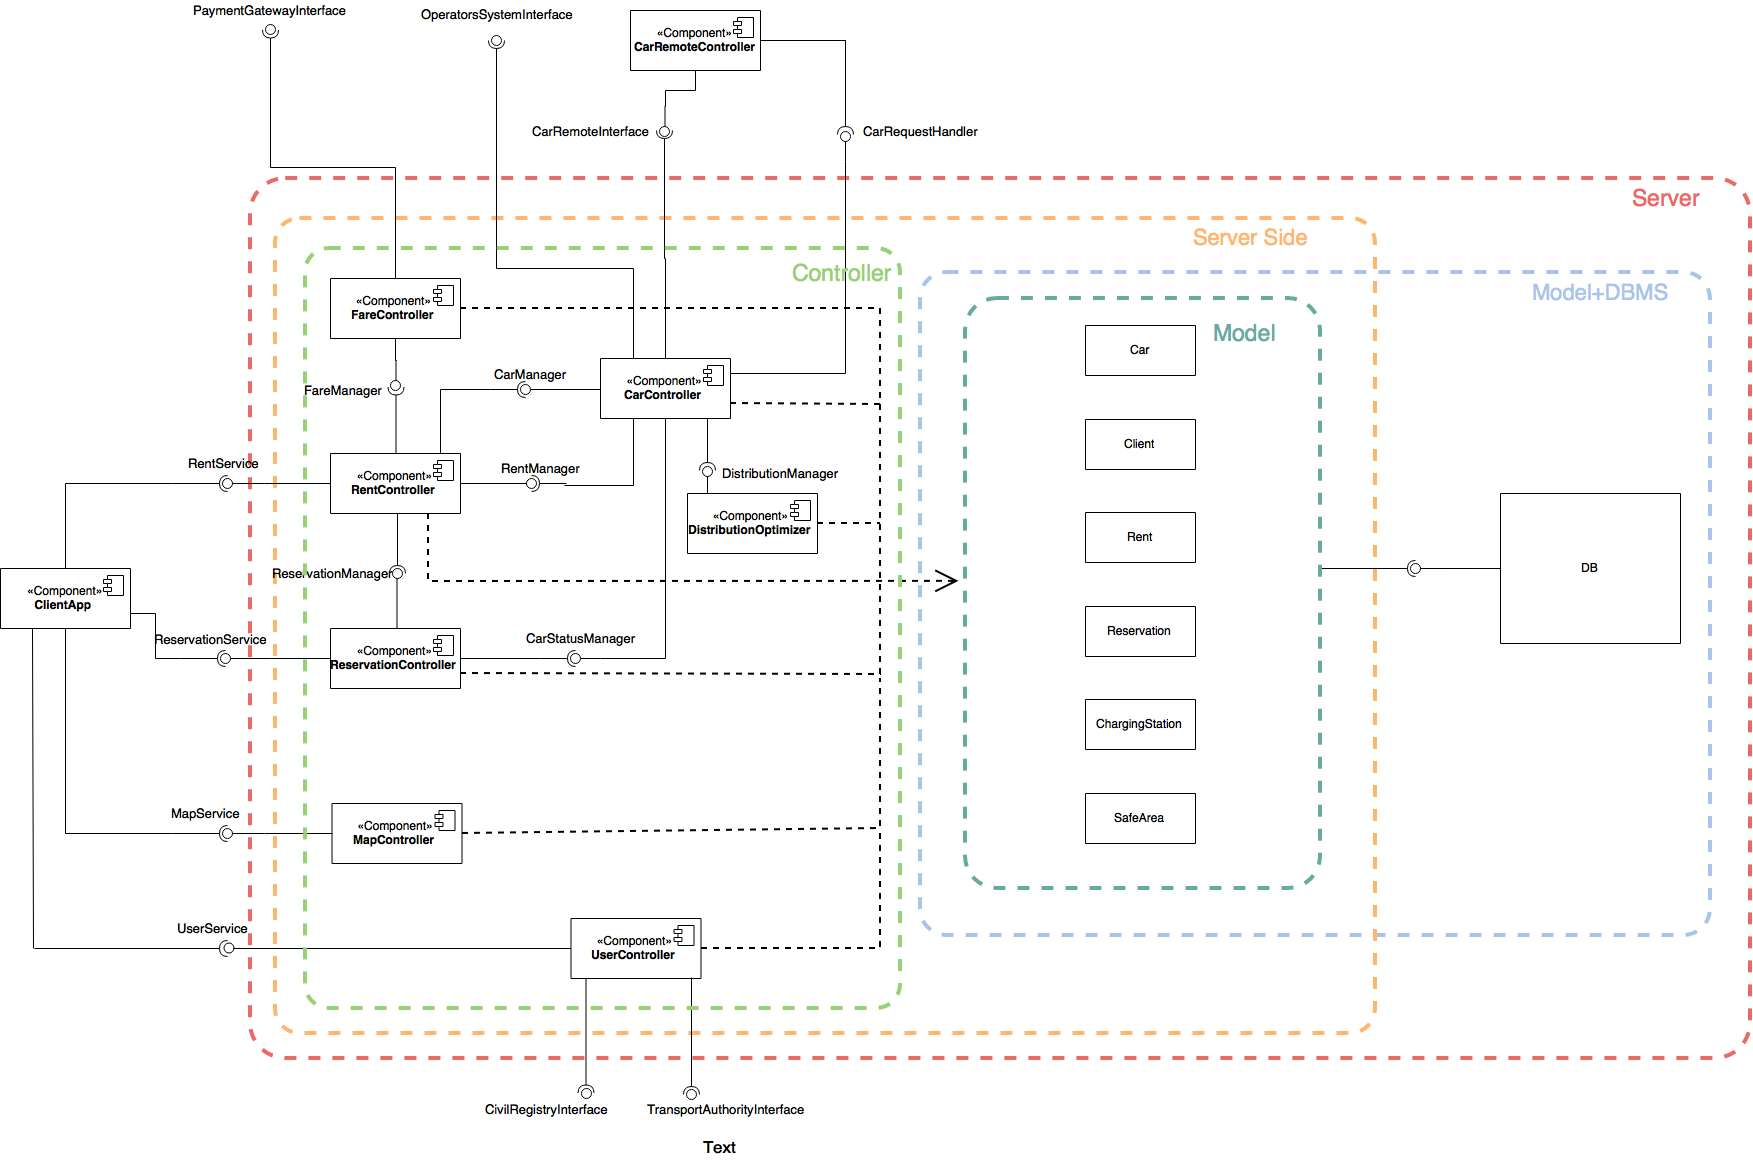
\includegraphics[width=450 pt]{resources/components.png}
\caption{\label{fig:component}Component diagram.}
\end{figure}
Starting from the components of the  diagram above we have identified the following subsystems :

\begin{itemize}
\item \textbf{Controller:} a set of all the controller components on the server side 
\item \textbf{Model:} composed by all the model components on the server side
\item \textbf{Model + DBMS} : composed by the Model and the DBMS 
\item \textbf{Server:} composed by the integration of the Controller with the subsystem Model+DBMS
\end{itemize}

The first integration is between the \textbf{Model} components, however the only interaction between them are getters and setters so we can integrate  all these components without testing them. From now on we will proceed  considering all the model components as an unique component named just \textbf{Model}. The next components to be integrated is the \textbf{DBMS} and the \textbf{Model}, obtaining a subsystem called \textbf{Model+DBMS}. 
Now we have to integrate the \textbf{Controller} components to the \textbf{Model+DBMS} subsystem. Then we can proceed to the integration between the controller components taking into account the yet succeeded integration between each of the \textbf{Controller} modules and the \textbf{Model+DBMS} subsystem. The result of this phase will be the \textbf{Server} subsystem. The next step is to integrate the  remaining standalone components : the \textbf{Client} and the \textbf{CarRemoteController}. In order to accomplish this task will be adopted a functional approach. 
We assume that the teams that will develop the components that use external services will test the external interfaces during the unit testing phase using some tools given by the service provider, so the integration of the external interfaces does not need to be tested again and they will be integrated directly to each component that makes use of them.

\newpage
\subsection{Integration testing strategy}
Due to the complexity of the project and the fact that it is deployed on several hardware devices we are going to use different integration testing approaches.
On a high level we are going to use a \textbf{bottom-up} approach to integrate the subsystems of \textbf{PowerEnjoy}. This incremental approach allows us to detect faster faults and bugs (compared to approaches like "big bang") and to evaluate easily the testing progress.
\begin{figure}[hp]
  \centering
  \includegraphics[width=200 pt]{resources/bottom_up_v2.png}
  \label{fig:bottom_up}
\end{figure}
\\
As written in the "Entry Criteria" all the components of the \textbf{Model} have already been tested and  they don't need integration testing because interacts only with getters and setters. 
Therefore we are going to consider the model as a unique component.\newline
The first step consist on the integration of the \textbf{Model} with the \textbf{DBMS} to test their interaction. \textbf{DBMS} is a commercial component that has already been developed so it can be immediately used in a bottom-up approach without any explicit dependency.
All the components of the \textbf{Controller} subsystem will be first integrated and tested with the \textbf{model} in order to facilitate future integration testing. This can be done separately and independently in order to save time.\newline
To integrate between them the components of the \textbf{Controller} subsystem we are going to 
use a "\textbf{Critical Module First}" approach. Starting from the riskiest and most connected parts will help us to detect bugs as soon as possible, but we will also need to develop some stubs and drivers.
We will start integrating CarController with :
\begin{itemize}
\item ReservationController
\item RentController
\item DistributionOptimizer
\end{itemize}
Also these integrations will be done independently using appropriate stubs and drivers.
We will procede integrating ReservationController with RentController and, after testing,integrating also FareController.

Once the Server has been fully tested, we are going to test the interaction between the three subsystems:
\begin{itemize}
\item ClientApp
\item CarRemoteController
\item Controller + Model + DBMS  (= Server)
\end{itemize}
In this phase a Big Bang approach would be too dispersive and would not guarantee a proper visibility on the functionalities because the system is big and presents complex interactions among his subsystems.
Even if the integration may result more complex, we opt for a \textbf{functional grouping} approach that will require less stubs/drivers and will provide better process visibility.
Portions of the different subsystems interact together to provide the following user-visible functions:
\begin{itemize}
\item Reservation
\item Start Rent
\item Map visualization
\item User Account Management
\item End Rent
\item Damage Report
\item MoneySavingOption Request
\end{itemize}
Another advantage of this approach is that functions can be tested separately and independently by different testing teams in order to speed up the testing process. 


\newpage

\subsection{Sequence of component/function integration}
In the following sub-paragraphs will be explain the order in which the tests between various components and subsystems will be performed. 

\subsubsection{Software integration sequence}

\begin{center}
\begin{tabular*}
{\textwidth}
{l p{8.5cm} l}
\hline
\textbf{ID} & \textbf{Integration Test} & \textbf{Paragraph} \\
\hline
I2T1 & (DBMS + Model) $\rightarrow$ MapController & 3.2\\
I2T2 & (DBMS + Model) $\rightarrow$ UserController & 3.2\\
I2T3 & (DBMS + Model) $\rightarrow$ CarController & 3.2\\
I2T4 & (DBMS + Model) $\rightarrow$ DistributionOptimizer & 3.2\\
I2T5 & (DBMS + Model) $\rightarrow$ ReservationController & 3.2\\
I2T6 & (DBMS + Model) $\rightarrow$ RentController & 3.2\\
I2T7 & (DBMS + Model) $\rightarrow$ FareController & 3.2\\
I3T1 &CarController$\rightarrow$ DistributionOptimizer & 3.3\\
I3T2 &CarController$\rightarrow$ ReservationController & 3.3\\
I3T3 &CarController$\rightarrow$ RentController & 3.3\\
I4T1 &ReservationController$\rightarrow$ RentController & 3.4\\
I5T1 &RentController$\rightarrow$FareController & 3.5\\
\hline
\newline
\newline
\end{tabular*}
\end{center}




As already mentioned, the integration between components follows a mix of bottom-up and critical-module-first approach. In the diagrams below, we focus on the component of the server side. The direction of the arrows indicates the order of integration. 
First of all, the model will be integrated with all controller component, and, for speed up this phase, this can be do in in parallel. This will allow every component to access to data needed for the other tests. On the next step we will integrate the components of the Controller subsystem. We will first integrate CarController with the interacting components: DistributionOptimizer
ReservationController, RentController.
Finally we will perform the  integration between ReservationController and RentController and between RentController and FareController .
The numbers that labels the edges indicate the sequence of integration. Notice that this order coincide with a topological order of the graph.

\begin{figure}[hp]
\centering
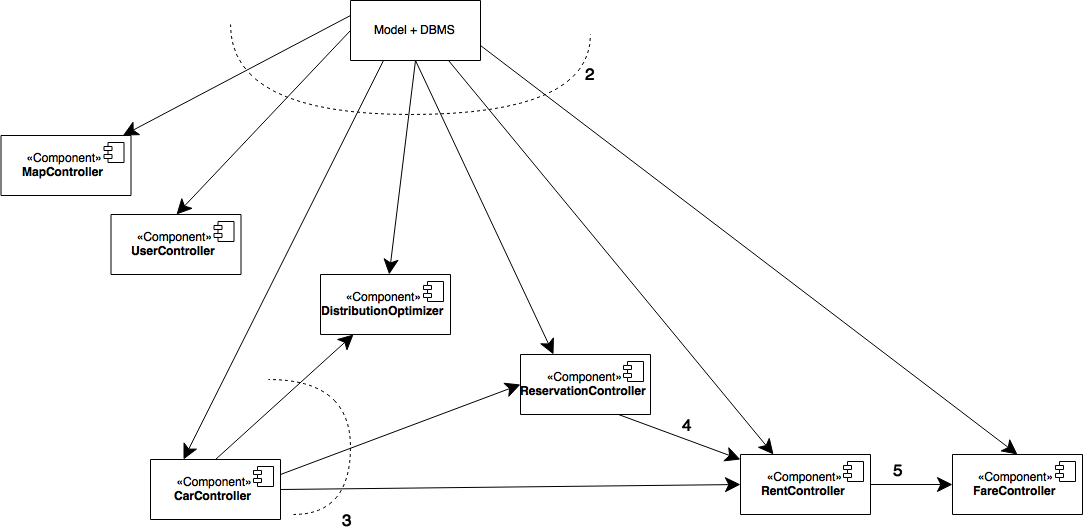
\includegraphics[width=470 pt]{resources/integrationServer.png}
\caption{\label{fig:IntServer}Integration strategy server side.}
\end{figure}


\subsubsection{Subsystem integration sequence}
\begin{center}
\begin{tabular*}
{\textwidth}
{l p{8.5cm} l}
\hline
\textbf{ID} & \textbf{Integration Test} & \textbf{Paragraph} \\
\hline
I1 & DBMS $\rightarrow$ Model & 3.1\\
I2 & (DBMS + Model) $\rightarrow$ Controller & 3.2\\
I6 & Client $\rightarrow$ Server $\rightarrow$ CarController & 3.6\\
\hline
\newline
\newline
\end{tabular*}
\end{center}

PowerEnJoy can be divided into different subsystems, as seen in Design document.
Since that the integration of the subsystems could hide various problems, we have decided to use a functional grouping approach. This strategy allows us to obtain a general view of the desired effects over the full system.

\begin{figure}[hp]
\centering
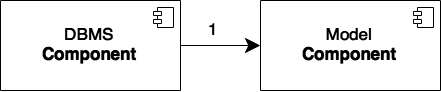
\includegraphics[width=150 pt]{resources/Model_+_DBMS.png}
\caption{\label{fig:Model+DBMS}Model + DBMS subsystem.}
\end{figure}

First of all, to make relevant all the following tests, we must test the integration between \textbf{DBMS} and \textbf{Model} subsystem. Then we focused on the \textbf{Controller} subsystem, as mentioned above, and integrate it with \textbf{DBMS + Model}. After that, we integrate the other server components. This integration has as result the \textbf{Server} subsystem. Finally the last integration will be between the Server subsystem and the remaining components :\textbf{CarController} and \textbf{ClientApp} .




\begin{figure}[hp]
\centering
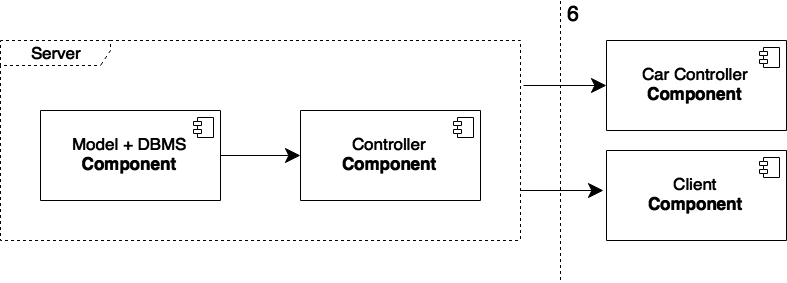
\includegraphics[width=400 pt]{resources/integrationSubSys.png}
\caption{\label{fig:SubSys}Integration strategy subsystem.}
\end{figure}



\newpage
\section{Individual steps and test description}
\subsection{Integration test case I1}
\begin{center}
\begin{tabular*}
{\textwidth}
{l p{10.5cm}}

\hline
\textbf{Test Case Identifier} & I1T1 \\
\hline
\textbf{Test Item(s)} &  Model and DBMS\\
\hline
\textbf{Input Specification} & Car,User,Rent,Reservation,ChargingStation,SafeArea\\
\hline
\textbf{Output Specification} & The Database queries are correctly called by the methods of the Model and there is referential integrity between the data in the database and the data of the model\\
\hline
\textbf{Environmental Needs} & N/A\\
\hline
\textbf{Dependencies} & Test data to fill the Database\\
\hline
\newline
\newline
\end{tabular*}
\end{center}


%----------------------------------------


\subsection{Integration test case I2}
\begin{center}
\begin{tabular*}
{\textwidth}
{l p{10.5cm}}
\hline
\textbf{Test Case Identifier} & I2T1 \\
\hline
\textbf{Test Item(s)} &  Model+DBMS and MapController  \\
\hline
\textbf{Input Specification} &  a gps position and a distance\\
\hline
\textbf{Output Specification} &  correct information about the indicated area like cars available, safe areas and charging stations\\
\hline
\textbf{Environmental Needs} & MapServiceDriver \\
\hline
\textbf{Dependencies} &  test data about map elements \\
\hline
\newline
\newline
\end{tabular*}
\end{center}

%--------------------------------------

\begin{center}
\begin{tabular*}
{\textwidth}
{l p{10.5cm}}

\hline
\textbf{Test Case Identifier} & I2T2 \\
\hline
\textbf{Test Item(s)} &  Model+DBMS and UserController  \\
\hline
\textbf{Input Specification} &  personal data and payment information in a correct format\\
\hline
\textbf{Output Specification} &  the system calls the right methods in order to insert the new user data into the database and allow the new user to use the service\\
\hline
\textbf{Environmental Needs} & UserServiceDriver \\
\hline
\textbf{Dependencies} &  N/A\\%DBMS stub\\
\hline
\newline
\newline
\end{tabular*}
\end{center}


%--------------------------------------


\begin{center}
\begin{tabular*}
{\textwidth}
{l p{10.5cm}}

\hline
\textbf{Test Case Identifier} & I2T3 \\
\hline
\textbf{Test Item(s)} &  Model+DBMS and CarController  \\
\hline
\textbf{Input Specification} &  Car, User\\
\hline
\textbf{Output Specification} &  The system invokes the right methods in order to change the car information in the model\\
\hline
\textbf{Environmental Needs} & CarManagerDriver, CarRequestHandlerDriver,  CarStatusManagerDriver\\
\hline
\textbf{Dependencies} &  CarRemoteController Stub,RentController Stub\\
\hline
\newline
\newline
\end{tabular*}
\end{center}


%--------------------------------------


\begin{center}
\begin{tabular*}
{\textwidth}
{l p{10.5cm}}

\hline
\textbf{Test Case Identifier} & I2T4 \\
\hline
\textbf{Test Item(s)} &  Model+DBMS and DistributionOptimizer  \\
\hline
\textbf{Input Specification} & gps position\\
\hline
\textbf{Output Specification} & The distributionOptimizer is able to get information about cars within a certain area\\
\hline
\textbf{Environmental Needs} &DistributionManagerDriver\\
\hline
\textbf{Dependencies} &  Test data about cars\\
\hline
\newline
\newline
\end{tabular*}
\end{center}



%--------------------------------------



\begin{center}
\begin{tabular*}
{\textwidth}
{l p{10.5cm}}

\hline
\textbf{Test Case Identifier} & I2T5 \\
\hline
\textbf{Test Item(s)} &  Model+DBMS and ReservationController  \\
\hline
\textbf{Input Specification} & Reservation, User, Car\\
\hline
\textbf{Output Specification} & The ReservationController invokes the right methods of the model in order to add a new reservation of the specified user for the specified car car\\
\hline
\textbf{Environmental Needs} & ReservationServiceDriver, ReservationManagerDriver\\
\hline
\textbf{Dependencies} &  test data about users and reservations, CarController stub\\ %DBMS stub, \\
\hline
\newline
\newline
\end{tabular*}
\end{center}

%--------------------------------------


\begin{center}
\begin{tabular*}
{\textwidth}
{l p{10.5cm}}

\hline
\textbf{Test Case Identifier} & I2T6 \\
\hline
\textbf{Test Item(s)} &  Model+DBMS and RentController  \\
\hline
\textbf{Input Specification} & Rent,Reservation, User, Car\\
\hline
\textbf{Output Specification} & The RentController invokes the right methods of the model in order to add a new rent of the specified user for the specified car preceded by the specified Reservation\\
\hline
\textbf{Environmental Needs} & RentServiceDriver , RentManagerDriver\\
\hline
\textbf{Dependencies} &  test data about rents and reservations and cars, FareControllerStub, CarControllerStub\\% DBMS stub,
\hline
\newline
\newline
\end{tabular*}
\end{center}


%--------------------------------------


\begin{center}
\begin{tabular*}
{\textwidth}
{l p{10.5cm}}

\hline
\textbf{Test Case Identifier} & I2T7 \\
\hline
\textbf{Test Item(s)} &  Model+DBMS and FareController  \\
\hline
\textbf{Input Specification} & Rent,User,Car\\ %  Per correttezza sarebbe client ma poi si confonde con il client  del client-server quindi magari si scrive nell'introduzione
\hline
\textbf{Output Specification} & The FareController acquire the needed information about the user \\
\hline
\textbf{Environmental Needs} & FareManagerDriver\\
\hline
\textbf{Dependencies} &  test data about users\\% DBMS stub,
\hline
\newline
\newline
\end{tabular*}
\end{center}


%--------------------------------------add

\subsection{Integration test case I3}
\begin{center}
\begin{tabular*}
{\textwidth}
{l p{10.5cm}}

\hline
\textbf{Test Case Identifier} & I3T1 \\
\hline
\textbf{Test Item(s)} &  CarController and DistributionOptimizer  \\
\hline
\textbf{Input Specification} & a gps area\\
\hline
\textbf{Output Specification} & The CarController invokes the right methods of DistributionOptimizer\\
\hline
\textbf{Environmental Needs} & I1T3 and I1T4 succeeded, CarRequestHandlerDriver\\
\hline
\textbf{Dependencies} &  Test Data about cars\\
\hline
\newline
\newline
\end{tabular*}
\end{center}


%--------------------------------------


\begin{center}
\begin{tabular*}
{\textwidth}
{l p{10.5cm}}

\hline
\textbf{Test Case Identifier} & I3T2 \\
\hline
\textbf{Test Item(s)} &  CarController and ReservationController  \\
\hline
\textbf{Input Specification} & Car\\
\hline
\textbf{Output Specification} & The ReservationController invokes the right methods of CarController in order to change the status of the specified car\\
\hline
\textbf{Environmental Needs} & I1T3 and I1T5 succeeded, ReservationServiceDriver\\
\hline
\textbf{Dependencies} &  CarRemoteController Stub\\
\hline
\newline
\newline
\end{tabular*}
\end{center}


%--------------------------------------


\begin{center}
\begin{tabular*}
{\textwidth}
{l p{10.5cm}}

\hline
\textbf{Test Case Identifier} & I3T3 \\
\hline
\textbf{Test Item(s)} &  CarController and RentController  \\
\hline
\textbf{Input Specification} & Car\\
\hline
\textbf{Output Specification} & The RentController invokes the right methods of CarController in order to unlock the doors of the specified car\\
\hline
\textbf{Environmental Needs} & I1T3 and I1T6 succeeded, RentServiceDriver,CarRequestHandlerDriver\\
\hline
\textbf{Dependencies} &  CarRemoteController Stub, FareControllerStub, ReservationControllerStub\\
\hline
\newline
\newline
\end{tabular*}
\end{center}


%--------------------------------------


\subsection{Integration test case I4}
\begin{center}
\begin{tabular*}
{\textwidth}
{l p{10.5cm}}

\hline
\textbf{Test Case Identifier} & I4T1 \\
\hline
\textbf{Test Item(s)} &  RentController and ReservationController   \\
\hline
\textbf{Input Specification} & Car,User,Reservation\\
\hline
\textbf{Output Specification} & The RentController invokes the right methods of ReservationController in order to modify the status of the reservation made by the specified user for the specified car\\
\hline
\textbf{Environmental Needs} & I1T5, I1T6, I2T2 and I2T3 succeeded, RentServiceDriver\\
\hline
\textbf{Dependencies} &  CarRemoteController Stub, FareController Stub,  test data about reservation, users and cars\\%DBMS stub,
\hline
\newline
\newline
\end{tabular*}
\end{center}


%--------------------------------------
\subsection{Integration test case I5}

\begin{center}
\begin{tabular*}
{\textwidth}
{l p{10.5cm}}

\hline
\textbf{Test Case Identifier} & I5T1 \\
\hline
\textbf{Test Item(s)} &  RentController and FareController   \\
\hline
\textbf{Input Specification} & Car,User,Rent\\
\hline
\textbf{Output Specification} & The RentController invokes the right methods of FareController in order to start the payment operations.\\
\hline
\textbf{Environmental Needs} & I1T6, I1T7, I2T3 and I3T1 succeeded,RentManagerDriver\\
\hline
\textbf{Dependencies} &   test data about rent and users\\%DBMS stub, \\
\hline
\newline
\newline
\end{tabular*}
\end{center}


%--------------------------------------




%Anto 
%--------------------------------------
\subsection{Integration test case I6: Reservation}

\begin{center}
\begin{tabular*}
{\textwidth}
{l p{10.5cm}}

\hline
\textbf{Test Case Identifier} & I6T1 \\
\hline
\textbf{Test Item(s)} & ClientApp and Server and CarRemoteController   \\
\hline
\textbf{Input Specification} & Client,Car \\
\hline
\textbf{Output Specification} & Server stores the request if all condition about client profile and car status are satisfied, then modify the status of the car invoking the right method of CarRemoteController and starts the reservation countdown.\\
\hline
\textbf{Environmental Needs} & I1...I5 succeeded. \\
\hline
\textbf{Dependencies} &  \\
\hline
\newline
\newline
\end{tabular*}
\end{center}


%--------------------------------------
\subsection{Integration test case I7: Start rent}

\begin{center}
\begin{tabular*}
{\textwidth}
{l p{10.5cm}}

\hline
\textbf{Test Case Identifier} & I7T1 \\
\hline
\textbf{Test Item(s)} & ClientApp and Server and CarRemoteController \\
\hline
\textbf{Input Specification} & Client,Car \\
\hline
\textbf{Output Specification} & The server checks if exist a valid reservation for (Client,Car) and after that, sends a remote command to the car to unlock the doors. \\
\hline
\textbf{Environmental Needs} &  I1...I5 succeeded. \\
\hline
\textbf{Dependencies} & N/A \\
\hline
\newline
\newline
\end{tabular*}
\end{center}

%--------------------------------------



%--------------------------------------
\subsection{Integration test case I8: Map visual}

\begin{center}
\begin{tabular*}
{\textwidth}
{l p{10.5cm}}

\hline
\textbf{Test Case Identifier} & I8T1 \\
\hline
\textbf{Test Item(s)} & ClientApp and Server \\
\hline
\textbf{Input Specification} & User, position \\
\hline
\textbf{Output Specification} & Server collects information about the available cars near the position, then send it to ClientApp.  \\
\hline
\textbf{Environmental Needs} &I1...I5 succeeded. \\
\hline
\textbf{Dependencies} & N/A\\
\hline
\newline
\newline
\end{tabular*}
\end{center}

%--------------------------------------


%--------------------------------------
\subsection{Integration test case I9: User Account Management}

\begin{center}
\begin{tabular*}
{\textwidth}
{l p{10.5cm}}

\hline
\textbf{Test Case Identifier} & I9T1 \\
\hline
\textbf{Test Item(s)} & ClientApp and Server \\
\hline
\textbf{Input Specification} & User\\
\hline
\textbf{Output Specification} & User submit his username and password, Server checks if the credentials are valid and allows the client to access to the system.   \\
\hline
\textbf{Environmental Needs} & I1...I5 succeeded. \\
\hline
\textbf{Dependencies} & N/A \\
\hline
\newline
\newline
\end{tabular*}
\end{center}

\begin{center}
\begin{tabular*}
{\textwidth}
{l p{10.5cm}}

\hline
\textbf{Test Case Identifier} & I9T2 \\
\hline
\textbf{Test Item(s)} & ClientApp and Server \\
\hline
\textbf{Input Specification} & User\\
\hline
\textbf{Output Specification} & User submit his personal data, the ClientApp checks if they are valid, the Server manages the request and register a new user.  \\
\hline
\textbf{Environmental Needs} &I1...I5 succeeded. \\
\hline
\textbf{Dependencies} & N/A \\
\hline
\newline
\newline
\end{tabular*}
\end{center}

%--------------------------------------

%
%--------------------------------------
\subsection{Integration test case I10: End rent}

\begin{center}
\begin{tabular*}
{\textwidth}
{l p{10.5cm}}

\hline
\textbf{Test Case Identifier} & I10T1 \\
\hline
\textbf{Test Item(s)} & Server and CarRemoteController \\
\hline
\textbf{Input Specification} & Request of end rent on CarRemoteController passing a GPS position that doesn't correspond to a safe area \\
\hline
\textbf{Output Specification} & The end of the rent is not allowed, is called a method on CarRemoteController that notifies the user on the car display.\\
\hline
\textbf{Environmental Needs} & I1...I5 succeeded. \\
\hline
\textbf{Dependencies} & N/A \\
\hline
\newline
\newline

\end{tabular*}
\end{center}

%--------------------------------------
\begin{center}
\begin{tabular*}
{\textwidth}
{l p{10.5cm}}

\hline
\textbf{Test Case Identifier} & I10T2 \\
\hline
\textbf{Test Item(s)} & Server and CarRemoteController \\
\hline
\textbf{Input Specification} & Request of end rent on CarRemoteController passing a GPS position corresponding to a safe area  \\
\hline
\textbf{Output Specification} & The right methods are called in CarRemoteController and in Server in order to : start the "lock doors" countdown, lock the car's doors, check if the car is plugged,save the rent information,calculate the discounts based, charge the client. \\
\hline
\textbf{Environmental Needs} &  I1...I5 succeeded.\\
\hline
\textbf{Dependencies} & N/A\\
\hline
\newline
\newline

\end{tabular*}
\end{center}

%--------------------------------------


%--------------------------------------
\subsection{Integration test case I11: Damage Report}

\begin{center}
\begin{tabular*}
{\textwidth}
{l p{10.5cm}}

\hline
\textbf{Test Case Identifier} & I11T1 \\
\hline
\textbf{Test Item(s)} & Server and CarRemoteController \\
\hline
\textbf{Input Specification} & Request of report damage/dirty car on the CarRemoteController\\
\hline
\textbf{Output Specification} & The right methods are called in CarRemoteController and in Server in order to: save the information of the report, acquire information about the current and previous rent and send them to the operator system,enable opportunity to end rent without charge. \\
\hline
\textbf{Environmental Needs} & I1...I5 succeeded.\\
\hline
\textbf{Dependencies} & N/A\\
\hline
\newline
\newline
\end{tabular*}
\end{center}
%--------------------------------------


%--------------------------------------
\subsection{Integration test case I12: MoneySavingOption Request}

\begin{center}
\begin{tabular*}
{\textwidth}
{l p{10.5cm}}

\hline
\textbf{Test Case Identifier} & I12T1 \\
\hline
\textbf{Test Item(s)} & CarRemoteController and Server \\
\hline
\textbf{Input Specification} & Request to enable "Money saving option" on the CarRemoteController passing the destination address \\
\hline
\textbf{Output Specification} & The right methods are called in CarRemoteController and in Server in order to calculate and return information about the charging station where to plug the car based on destination address,cars distribution,charging spots availability.  \\
\hline
\textbf{Environmental Needs} & I1...I5 succeeded. \\
\hline
\textbf{Dependencies} & N/A\\
\hline
\newline
\newline
\end{tabular*}
\end{center}

%--------------------------------------

\newpage
\section{Tools and test equipment required}
In order to simplify and speed up the testing phase, we are going to use some automated tools.
Furthermore, the test must be run in a specific environment with a reasonable data, these must approximate as much as possible the expected reality.

\subsection{Tools}

For testing the business logic, that could be written in Java EE, we can use two main tools that work together, \textbf{Arquillan} and \textbf{JUnit}.\\
Arquillan is a tool that help to verify the correct interaction between a component and its execution environment. Therefore we will use this tools in order to identify eventually problems into a Java container that has deployed on server side. More precisely, we check the right component injection where another component need them.\\
Even if JUnit framework is used during unit test, it can be also used as support to verify that during an interaction between components the right effect will be produced. For example, we use it to check that the correct object is returned when a method is invoked or to assure that an exception is raised when the invoked method is invalid.\\
Finally one other tool that can be useful is \textbf{Mockito}. This tool help us to create the stub necessary during the integration test. In particular, when a component to be called isn't yet implemented, Mockito easily allows us to define a fake response for the caller.\\
Furthermore, particularity attention will be posed on the performance that the system should be guarantee during certain phase. For example, it's requested a high reactivity during the operation of start a rent and end a rent. For this purpose we can use \textbf{JMeter}, that allows us to load the system with a reasonable quantity of request and verify that the system performance meets a certain criteria of performance.


\subsection{Test equipment required}

In order to perform a valid integration tests, an environment with a minimum specific requirement is needed.
The PowerEnJoy system is made up by a different types of hardware component, so during the test phase it's required an heterogeneous representation of them. 
Surely, in addition to server and database that constitute the core of the system, is required a car provided by equipment necessary to interact and communicate remotely. 
The most critical aspect is represented by the choice of the client device. In fact, if for testing the web application can be used a little set of the most used browser, for the mobile app it's necessary to use more configurations. For a minimum coverage of possible real situations is requested at least one mobile device for each OS, and it's recommended to use different display size. 
Finally should be recreated special situations like for example those in which there is low data connectivity or the GPS signal is absent.


\newpage
\section{Program stubs and test data required}
\subsection{Stubs}
Since we are using a critical-first strategy we need  5 stubs:

\subsubsection{CarRemoteControllerStub}
\textbf{Usages:}
\begin{itemize}
\item I2T3
\item I3T2
\item I3T3
\item I4T1
\end{itemize}

\textbf{Description}
This stub emulates the behavior of the car system, it is used by the CarController to achieve several tasks:
\begin{itemize}
\item Updating periodically the car position in the model
\item Opening and closing the car doors after a client request
\item Changing the car status
\end{itemize}

\subsubsection{CarControllerStub}
\textbf{Usages:}
\begin{itemize}
\item I2T5
\item I2T6
\end{itemize}

\textbf{Description}
This stub emulates the behavior of the CarController component, it is used by the ReservationController  to check and eventually change the car status after a new request of rent or reservation.

\subsubsection{FareControllerStub}
\textbf{Usages:}
\begin{itemize}
\item I2T6
\item I3T3
\item I4T1
\end{itemize}
\textbf{Description}
This stub emulates the behavior of the FareController component, it is used by the RentController to  make a payment request and verify that the payment succeed after an end rent request.

\subsubsection{RentControllerStub}
\textbf{Usages:}
\begin{itemize}
\item I2T3
\end{itemize}

\textbf{Description}
This stub emulates the behavior of the RentController component, it is used by the CarController to end a rent after receiving an end rent  request.

\subsubsection{ReservationControllerStub}
\textbf{Usages:}
\begin{itemize}
\item I3T3
\end{itemize}

\textbf{Description}
This stub emulates the behavior of the ReservationController component, it is used by the RentController to verify the existence of a valid reservation after receiving  a start rent  request .

\subsection{Drivers}
Since we are using a bottom-up approach we will need several Divers in order to accomplish our integration tests, here there is a list of drivers with their functionalities:

\begin{itemize}
\item \textbf{MapServiceDriver}: used in the test \textbf{I2T1},  this driver calls the methods of the \textbf{MapController} in order to test its integration with the \textbf{Model}, mostly are getters methods, to get the information about a certain area or about cars.
\item \textbf{UserServiceDriver}: used in the test \textbf{I2T2},  this driver calls the methods of the \textbf{UserController} in order to test its integration with the \textbf{Model}, this driver have to emulate a user that try to register or log in to \textbf{PowerEnjoy}, so it has to enter some personal data calling the right methods of \textbf{UserController}.
\item \textbf{CarManagerDriver}: used in the test \textbf{I2T3},  this driver calls the methods of the \textbf{CarController} in order to test its integration with the \textbf{Model} . The driver has to emulate the environment of a new rent request, made by the \textbf{RentController}
\item \textbf{CarRequestHandlerDriver}: used in the test \textbf{I2T3},  this driver calls the methods of the \textbf{CarController} in order to test its integration with the \textbf{Model}. The driver has to emulate the environment of a end rent request, emulating the behavior of the \textbf{CarRemoteController}.
\item \textbf{CarStatusManagerDriver}: used in the test \textbf{I2T3},  this driver calls the methods of the \textbf{CarController} in order to test its integration with the \textbf{Model}. The driver has to emulate the environment of a new Reservation request, emulating the behavior of the \textbf{ReservationController}.
\item \textbf{DistributionManagerDriver}: used in the test \textbf{I2T4},  this driver calls the methods of the \textbf{DistributionOptimizer} in order to test its integration with the \textbf{Model}. The driver emulate the environment of a request of a possible car distribution made by the \textbf{CarController}
\item \textbf{ReservationServiceDriver}: used in the tests \textbf{I2T5} ,\textbf{I3T2}  this driver calls the methods of the \textbf{ReservationController} in order to test its integration with the \textbf{Model} and with the \textbf{CarController}. It emulates the behavior of a client that tries to do a reservation on a car.
\item  \textbf{ReservationManagerDriver}: used in the test \textbf{I2T5}  this driver calls the methods of the \textbf{ReservationController} in order to test its integration with the \textbf{Model}.It emulates the behavior of  \textbf{RentController} when it receives an new rend request. 
\item \textbf{RentServiceDriver}: used in the tests \textbf{I2T6}, \textbf{I3T3}, \textbf{I4T1} and \textbf{I5T1}  this driver calls the methods of the \textbf{RentController} in order to test its integration with the Model, with the \textbf{CarController}, with \textbf{ReservationController} and with the \textbf{FareController}.It emulates the behavior of a client that tries to rent a car he has previously reserved .
\item \textbf{RentManagerDriver}: used in the test \textbf{I2T6}  this driver calls the methods of the \textbf{RentController} in order to test its integration with the \textbf{Model}.It emulates the behavior  \textbf{CarController} when it receives an end rend request. 
\item \textbf{FareManagerDriver}: used in the test \textbf{I2T7},  this driver calls the methods of the \textbf{FareController} in order to test its integration with the \textbf{Model}.It emulates the behavior of  \textbf{RentController} when it receives an end rend request. 
\item \textbf{CarRequestHandlerDriver}: used in the tests \textbf{I3T1} and \textbf{I3T3},  this driver calls the methods of the \textbf{CarController} in order to test its integration with the \textbf{DistributionOptimizer} and \textbf{RentController}. It emulates the requests made by \textbf{CarRemoteController}. 
\end{itemize}


\subsection{Test Data}
In order to produce some significant tests we  will need to populate our database with several fake data  for users, requests(past and running),rents(past and running), charging stations, cars, map and all other entities that will populate the database. 
The generation of such data can be made using some faker library that will allow us to populate the database.



\newpage
\section{Effort spent}
During the whole project the team worked with the following schedule:\\ \emph{\\}
\textbf{Claudio Salvatore Arcidiacono}
\begin{itemize}
\item 9 January  : 16.30-20.30 4 hours
\item 10 January : 16.30-20.30 4 hours
\item 12 January : 17-20 3 hours
\item 13 January : 11-13 2 hours
\item 13 January : 15-18 3 hours 
\item 14 January : 17-20 3 hours
\item 15 January : 17-20 3 hours\\

\textbf{Total hours:} 22 hours.
\end{itemize}


\textbf{Antonio Di Bello}
\begin{itemize}
\item 9 January  : 4 hours
\item 10 January : 4 hours
\item 12 January : 2 hours
\item 13 January : 2 hours
\item 14 January : 6 hours 
\item 15 January : 3 hours \\

\textbf{Total hours:} 21 hours.
\end{itemize}


\textbf{Denis Dushi}
\begin{itemize}
\item 9 January  :  4 hours
\item 10 January :  4 hours
\item 12 January :  3 hours
\item 13 January :  2 hours
\item 14 January :  6 hours
\item 15 January :  7 hours\\

\textbf{Total hours:} 26 hours.
\end{itemize}

\newpage
\section{References}
\subsection{Software and tool used}
The tools we used to create this document are:
\begin{itemize}
\item Overleaf (for latex writing in parallel)
\end{itemize}

\end{document}